% ReproLab Paper-001 preprint — v0 draft
% Target: arXiv cond-mat.mtrl-sci (cross-list: cs.LG)
% TODO(user): confirm author name romanization and affiliation line before submission.
% Build: tectonic main.tex
\documentclass[11pt]{article}

\usepackage[a4paper,margin=2.7cm]{geometry}
\usepackage{amsmath}
\usepackage{booktabs}
\usepackage{graphicx}
\usepackage{microtype}
\usepackage[hidelinks]{hyperref}
\usepackage{caption}
\captionsetup{font=small,labelfont=bf}

\newcommand{\code}[1]{\texttt{#1}}
\newcommand{\meV}{\,meV/atom}
\setlength{\emergencystretch}{2em}

\title{An Independent Reproducibility Audit of the\\Matbench Discovery Benchmark}
\author{Koju Maruyama\\
\normalsize ReproLab (independent)\\
\normalsize \href{mailto:info@marubo.biz}{info@marubo.biz}}
\date{July 2026 --- v0 draft}

\begin{document}
\maketitle

\begin{abstract}
Leaderboards increasingly mediate progress in machine learning for materials
science, yet they are rarely subjected to independent, execution-level
verification. We audit Matbench Discovery, a widely used benchmark ranking
machine-learning interatomic potentials on crystal stability prediction, at
three layers. \textbf{Layer A (metric recomputation):} for four released models
(CHGNet, SevenNet-0, MACE-MP-0, ORB v2) every published discovery metric
reproduces exactly from the released prediction files and bundled ground truth
--- every fraction to three decimals and every integer confusion count, via both
a from-scratch reimplementation and the upstream metric code.
\textbf{Layer B (prediction regeneration):} rerunning the three
relaxation-based models on a deterministic 500-structure subset reproduces the
released predictions to a median $|\Delta e_\mathrm{form}|$ of
0.03--0.05\meV{} with 99.6--100\% stability-classification agreement, across a
2023$\to$2026 dependency gap. \textbf{Layer C (statistical and provenance
audit):} the leaderboard reports no uncertainty; paired bootstrap confidence
intervals of $\pm$0.003--0.004 F1 imply that 43 of 59 adjacent pairs on the
60-model leaderboard are closer than one CI width. The three MPtrj-trained
models share failure modes (error correlation $r\approx0.76$; joint-miss rate
25$\times$ the independence prediction). Separately, the benchmark's
ground-truth stability column depends on the pymatgen version through MP2020
anion-correction assignment: pymatgen 2023.5.10 reproduces all audited values,
while 2026.5 shifts 3 of 500 by 119--217\meV{} and flips two labels ---
demonstrated bidirectionally with a version-pinned control environment. The
audit produced two upstream issue reports and a merged fix (checksum
verification; matbench-discovery PR~\#359). Our results support the
benchmark's headline conclusions while showing concretely where independent
verification breaks down, and suggest that leaderboards report uncertainty and
pin ground-truth provenance as a matter of course.
\end{abstract}

\section{Introduction}

Benchmarks and their leaderboards have become the primary interface through
which progress in machine learning for science is claimed, compared, and
consumed. In materials discovery, Matbench Discovery~\cite{riebesell2025}
ranks machine-learning interatomic potentials (MLIPs) by their ability to
classify the thermodynamic stability of $\sim$257{,}000 candidate crystal
structures from the WBM dataset~\cite{wang2021wbm}, and its public leaderboard
is a de facto reference for model selection in the field.

The reliability of such leaderboards is usually argued from internal
consistency: the maintainers run the evaluation code, and submitters
provide predictions in good faith. What is missing is \emph{independent,
execution-level} verification --- a third party, starting from only the public
code, data, and model checkpoints, attempting to reproduce the published
numbers and documenting exactly where the pipeline resists reproduction. Such
audits are routine in other empirical sciences and increasingly urged for
machine-learning research~\cite{kapoor2023}, but they are rarely performed for
AI-for-science benchmarks, plausibly because a full rerun appears to require
prohibitive compute.

This paper reports such an audit of Matbench Discovery, and makes three
methodological points that generalize beyond this one benchmark:

\begin{enumerate}
\item \textbf{A benchmark decomposes into independently checkable layers with
very different costs.} Verifying that published metrics follow from published
predictions (Layer A) is deterministic and takes CPU-minutes. Verifying that
the predictions themselves regenerate from model execution (Layer B) needs a
GPU but is meaningful on a small deterministic subset with pre-registered
acceptance thresholds. Statistical resolution and ground-truth provenance
(Layer C) require no new model execution at all.
\item \textbf{The audit is informative in both directions.} Matbench
Discovery passes Layers A and B cleanly --- a substantive positive finding that
strengthens the benchmark --- while Layer C surfaces two structural issues
invisible from inside the leaderboard: unreported statistical resolution, and
ground truth that silently depends on a library version.
\item \textbf{Audits can feed fixes upstream.} The operational findings led
to two upstream issues and a merged pull request (janosh/matbench-discovery
\#359, merged 2026-07-04) adding download checksum verification and repairing
stale checksums, closing the loop from audit to benchmark improvement.
\end{enumerate}

All commands, environments, and intermediate artifacts are logged in the audit
repository,\footnote{\url{https://github.com/maruyamakoju/reprolab}, release
\code{v0.4-external-handoff}.} and every reported number traces to a specific
script and data file.

\section{Audit design}

\paragraph{Object under audit.} Matbench Discovery at repository commit
\code{eaa7550} (package version 1.3.1), discovery task only: given a
structure's predicted formation energy, classify it stable or unstable
relative to the Materials Project convex hull ($E_\mathrm{hull}=0$ threshold),
scored by F1, precision, recall, accuracy, MAE, RMSE, $R^2$, and confusion
counts on two published subsets (\code{full\_test\_set}, $n=256{,}963$;
\code{unique\_prototypes}, $n=215{,}488$).

\paragraph{Three layers.}
\begin{itemize}
\item \textbf{Layer A --- metric recomputation (deterministic, CPU).} For each
model, recompute all discovery metrics from the released prediction CSV and the
bundled WBM ground truth, two independent ways: a from-scratch
reimplementation written for this audit, and the upstream
\code{stable\_metrics} function. Diff both against the official values
committed in the model's YAML file (the leaderboard's source of truth).
\item \textbf{Layer B --- prediction regeneration (GPU, subset).} Rerun the
model itself --- initial structure $\to$ FIRE relaxation under the
model-specific published protocol $\to$ formation energy --- on a deterministic
500-structure subset (seed-42 sample of \code{unique\_prototypes}; structure
ids committed to the repository), and score the regenerated predictions
through the identical Layer A path. Acceptance thresholds were pre-registered
before the first GPU run: median $|\Delta e_\mathrm{form}| \le 10$\meV{}
against the released predictions and $\ge$95\% stability-classification
agreement.
\item \textbf{Layer C --- statistical and provenance audit (CPU).}
(i) Quantify the statistical resolution of the leaderboard via paired
bootstrap over structures ($B=2000$), threshold sensitivity, and inter-model
error correlation. (ii) Recompute the ground-truth
$E_\mathrm{hull}$ column from the published computed-structure entries, the
MP2020 correction scheme~\cite{wang2021corrections}, and the published 2023
phase diagram, under two pymatgen~\cite{ong2013} versions. Layer C analyses
are exploratory (not pre-registered), and we label them as such.
\end{itemize}

\paragraph{Environment.} Windows 11, Python 3.11.9, single RTX 4090,
PyTorch 2.11.0+cu128; full \code{pip freeze} and per-command logs in the
repository. The audited models are CHGNet~\cite{deng2023},
SevenNet-0~\cite{park2024}, MACE-MP-0~\cite{batatia2024}, and
ORB v2~\cite{neumann2024}, spanning three architecture families and the
leaderboard F1 range 0.61--0.88.

\section{Layer A: published metrics reproduce exactly}

\begin{table}[t]
\centering
\small
\caption{Layer A --- official vs.\ recomputed discovery metrics
(\code{unique\_prototypes} subset). Official values from each model's
committed YAML; recomputed values agree via both the from-scratch and the
upstream implementation. Confusion counts (TP/FP/TN/FN) are integer-exact for
all four models on both subsets; \code{full\_test\_set} results (not shown)
are likewise exact.}
\label{tab:layer-a}
\begin{tabular}{lcccc}
\toprule
Model & F1 (official) & F1 (recomputed) & MAE eV/atom (off.) & MAE (recomp.) \\
\midrule
CHGNet     & 0.613 & 0.613 & 0.063 & 0.063 \\
SevenNet-0 & 0.724 & 0.724 & 0.048 & 0.048 \\
MACE-MP-0  & 0.669 & 0.669 & 0.057 & 0.057 \\
ORB v2     & 0.880 & 0.880 & 0.028 & 0.028 \\
\bottomrule
\end{tabular}
\end{table}

For all four models and both subsets, every published fraction reproduces to
all three published decimals and every confusion-matrix count is
integer-exact (Table~\ref{tab:layer-a}). The outlier-handling paths also
reproduce in both regimes the data exercises: the $|\Delta e| > 5$~eV/atom
error filter (CHGNet 2, SevenNet-0 3, ORB v2 2 structures dropped) and
genuine missing predictions (MACE-MP-0: 38 on \code{full\_test\_set}, 34 on
\code{unique\_prototypes}). The from-scratch reimplementation and the upstream
metric function never disagreed, so the leaderboard's metric code is faithful
to its stated definitions.

This is the cleanest possible outcome for the benchmark, and it is not vacuous:
Layer A is precisely where silent errors in data joins, subset masks, NaN
handling, and rounding conventions would surface.

\section{Layer B: released predictions regenerate from model execution}

For the three relaxation-based models we regenerated predictions from scratch
on the committed 500-structure subset, using each model's published protocol
(FIRE optimizer, $\le$500 steps, \code{FrechetCellFilter}; model-specific
force-convergence threshold $f_\mathrm{max}$), and scored them through the
unchanged Layer A path.

\begin{table}[t]
\centering
\small
\caption{Layer B --- regenerated vs.\ released formation energies on the
committed $n{=}500$ subset. Pre-registered thresholds: median
$|\Delta| \le 10$\meV{}, classification agreement $\ge$95\%. All runs:
500/500 structures relaxed, zero failures, single RTX 4090.}
\label{tab:layer-b}
\begin{tabular}{lccccc}
\toprule
Model & median $|\Delta|$ & p95 & max (\meV) & class.\ agreement & GPU time \\
\midrule
CHGNet    & 0.03 & 0.07 & 1.08   & 100\% (0 flips) & 9.3 min \\
MACE-MP-0 & 0.03 & 0.06 & 216.65 & 99.6\% (2 flips) & 10.1 min \\
ORB v2    & 0.05 & 0.17 & 16.86  & 100\% (0 flips) & 5.2 min \\
\bottomrule
\end{tabular}
\end{table}

All three models pass the pre-registered criteria by two to three orders of
magnitude (Table~\ref{tab:layer-b}). Three observations qualify the headline:

\paragraph{Reproduction survives a large dependency gap.} The released CHGNet
predictions were generated circa 2023 (torch 1.11, ase 3.22); we regenerated
them under torch 2.11 and ase 3.29 with the same 0.3.0 weights (412{,}525
parameters verified) and matched to a median of 0.03\meV{} --- below the
rounding scale of the released CSVs. GPU run-to-run variance, bounded on a
20-structure two-run control, is median 0.000 / max 0.232\meV, so the deltas
are interpretable.

\paragraph{The large MACE deviations are the ground truth's, not the
model's.} MACE-MP-0's three large outliers (up to 216.65\meV) are exactly the
three structures independently isolated by the Layer C ground-truth audit as
MP2020 correction-version drift cases (Section~\ref{sec:gt}); outside them,
regenerated MACE predictions match at rounding scale. Of its two
classification flips, one is a 0.1\meV{} threshold-boundary case.

\paragraph{Protocol ambiguity is a real failure mode.} ORB v2 reproduced
only under the force threshold recorded in its model YAML
($f_\mathrm{max}=0.02$); the upstream runner script's default (0.05) produced
a 212\meV{} error and a classification flip already at the two-structure
pre-check. Where a repository ships both a runner default and a per-model
YAML value, the YAML is authoritative --- but nothing in the pipeline says so,
and an independent reproducer who trusts the runner script fails.

Layer B is a subset audit of the generation path, not a full leaderboard
rerun; we return to this in Limitations.

\section{Layer C: statistical resolution of the leaderboard}
\label{sec:stats}

The leaderboard publishes point estimates only. We quantify what they resolve,
using the exact evaluation path validated in Layer A
(\code{unique\_prototypes}, $n=215{,}488$; paired bootstrap over structures,
$B=2000$).

\begin{table}[t]
\centering
\small
\caption{Paired-bootstrap 95\% confidence intervals for the four audited
models. All six pairwise F1 orderings among these four are stable
($P(\mathrm{flip})=0$ across 2000 resamples).}
\label{tab:ci}
\begin{tabular}{lcccc}
\toprule
Model & F1 & 95\% CI & CI width & MAE eV/atom [95\% CI] \\
\midrule
ORB v2     & 0.8801 & [0.8775, 0.8827] & 0.0052 & 0.0282 [0.0279, 0.0285] \\
SevenNet-0 & 0.7244 & [0.7207, 0.7281] & 0.0074 & 0.0484 [0.0481, 0.0487] \\
MACE-MP-0  & 0.6695 & [0.6657, 0.6733] & 0.0076 & 0.0569 [0.0566, 0.0573] \\
CHGNet     & 0.6126 & [0.6087, 0.6165] & 0.0078 & 0.0635 [0.0631, 0.0638] \\
\bottomrule
\end{tabular}
\end{table}

\begin{figure}[t]
\centering
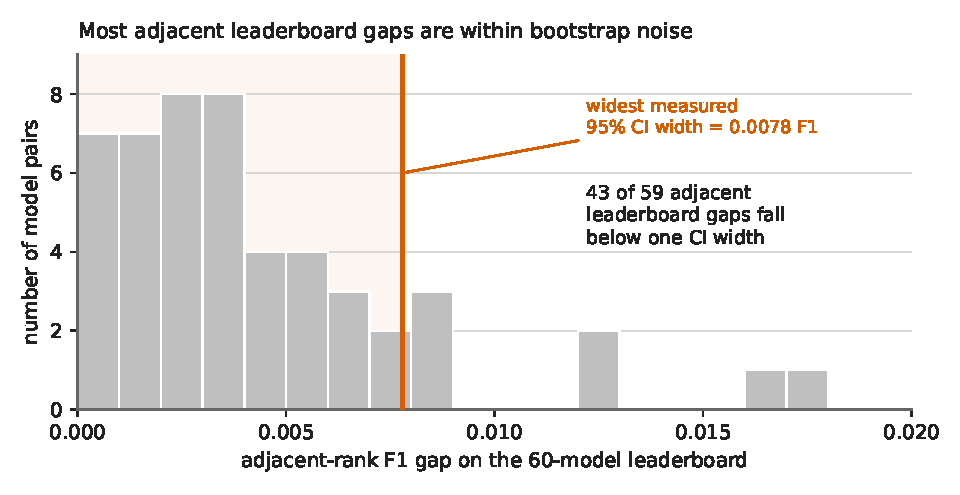
\includegraphics[width=0.82\textwidth]{fig_resolution.pdf}
\caption{Distribution of the 59 adjacent-rank F1 gaps on the full 60-model
\code{unique\_prototypes} leaderboard (gaps recomputed from the committed model
YAMLs), against the widest paired-bootstrap 95\% CI width measured among the
four audited models (0.0078 F1; Table~\ref{tab:ci}). Forty-three of the 59
gaps --- most of the leaderboard --- fall below one CI width, so neighboring
ranks are largely within the statistical noise the leaderboard does not
report.}
\label{fig:resolution}
\end{figure}

\paragraph{The audited models are cleanly separated; much of the leaderboard
is not.} The four audited models' F1 confidence intervals are
$\pm$0.003--0.004 wide and their six pairwise orderings never flip in 2000
paired resamples (Table~\ref{tab:ci}). But at the full leaderboard (60 models
with a \code{unique\_prototypes} F1 at this commit), \textbf{43 of 59
adjacent-rank gaps are smaller than the widest measured CI width (0.0078
F1)} (Figure~\ref{fig:resolution}); many are 0.000--0.003. The published
ordering among neighboring models
is therefore unlikely to be statistically resolvable without paired
significance testing --- which the per-structure prediction files, to the
benchmark's credit, make possible. (Caveat: CI width varies by model; a
definitive per-pair statement requires the paired bootstrap on each pair's
prediction files, as done here for four models.)

\paragraph{The ranking is threshold-robust.} A sweep of the stability
threshold from $-100$ to $+100$\meV{} (17 values, applied to truth and
prediction alike) leaves the four audited models' ranking unchanged at every point ---
relevant because DFT hull energies themselves carry uncertainty on the order
of 10\meV.

\paragraph{Training-data lineage, not just rank, drives discovery value.}
Signed formation-energy errors of the three MPtrj-trained models (CHGNet,
SevenNet-0, MACE-MP-0) are strongly correlated (Pearson $r=0.764$--$0.765$
pairwise), while ORB v2 (trained on additional data) correlates at only
$r=0.43$--$0.51$ with them. Of 33{,}374 DFT-stable structures, 3.59\% are
missed by all four models simultaneously --- 25$\times$ the 0.14\% expected
under error independence (12$\times$ within the near-hull band
$|E_\mathrm{hull}| \le 50$\meV). ORB v2 contributes 1{,}886 unique true
positives (stable materials found by it alone among the four), versus 341--388
for each of the others. For a practitioner running several models to triage
candidates, ensemble diversity is quantifiably more valuable than adjacent
leaderboard rank.

\section{Layer C: ground truth depends on the pymatgen version}
\label{sec:gt}

The benchmark's ground-truth column
(\code{e\_above\_hull\_mp2020\_corrected\_ppd\_mp}) is distributed as a
precomputed artifact. We recomputed it for the 500 audited structures from the
published computed-structure entries, the MP2020 correction
scheme~\cite{wang2021corrections}, and the published 2023
\code{PatchedPhaseDiagram}, under pymatgen 2026.5:

\begin{itemize}
\item 497/500 values reproduce to $\le 0.001$\meV{} (median
$|\Delta| = 0.0003$\meV);
\item 3/500 shift by 119--217\meV, flipping two stability labels
(SrBrN$_3$, PaIO, NdH$_4$Pt);
\item for all three, the $E_\mathrm{hull}$ discrepancy equals the formation
energy discrepancy to $<0.001$\meV{} --- the phase-diagram lookup is not
implicated; the entire difference is in MP2020 anion-correction
\emph{assignment}, which hinges on pymatgen's oxidation-state guessing
heuristics (e.g., whether SrBrN$_3$ receives a nitride correction in addition
to the bromide one, or whether NdH$_4$Pt receives a hydride correction at
all).
\end{itemize}

\paragraph{Bidirectional demonstration.} In a control environment pinned to
pymatgen 2023.5.10 --- the version referenced by the benchmark's own data
manifest --- the identical recomputation reproduces the published values for
all three outliers to $\le 0.031$\meV{} (and 500/500 overall). The published
column is thus internally consistent \emph{with respect to a specific,
unstated library version}: correct under 2023.5.10, unreproducible under
2026.5, in both directions traceable to the same correction-assignment code
paths.

Which correction assignment is chemically preferable is out of scope. The
reproducibility point is sharper: a benchmark's ground truth embedded
heuristic decisions of a specific library version without recording that
dependency, and $\sim$0.5\% label ambiguity is material on a leaderboard
where adjacent models are separated by $\Delta$F1 of 0.001--0.003
(Section~\ref{sec:stats}). Following our report, a provenance note was folded
into the upstream fix (PR~\#359).

\section{Operational reproducibility findings}

Four operational findings, each invisible to users of the maintainers' own
pipeline and encountered only on the independent-reproduction path:

\begin{enumerate}
\item \textbf{Stale and missing checksums, and no verification.} The
upstream MD5 recorded for the WBM initial-structures file belonged to an
older artifact in the same Figshare deposit (two other files had no recorded
checksum), and the download path never verified checksums, so the errors were
latent. Reported as issues \#357/\#358; fixed by our
PR~\#359 (merged 2026-07-04), which repairs the checksums and adds
verification at download time.
\item \textbf{Landing-page URLs are WAF-blocked for scripted downloaders.}
The recorded \code{figshare.com/files/<id>} URLs return an empty body to a
plain GET; the API endpoint works. The package rewrites URLs internally, so
only independent tooling hits this.
\item \textbf{The PyPI wheel and the repository differ under the same
version string} (1.3.1): flat module layout on PyPI vs.\ package layout at
HEAD, with different import paths. \code{pip install} alone does not
reproduce the repository's evaluation entrypoints; we audited the pinned
clone.
\item \textbf{Dependency drift breaks config loading}: ruamel.yaml 0.19 with
current pymatgen/monty fails with an opaque error; pinning
\code{ruamel.yaml<0.19} resolves it.
\end{enumerate}

\section{Limitations}

Layer B covers three models on 500 of 257k structures --- a deliberate,
deterministic subset with pre-registered thresholds, not a full leaderboard
regeneration; SevenNet-0 was audited at Layer A only. Only the discovery task
was audited (not phonons, geometry, or diatomics). All runs used a single
environment (Windows 11, one RTX 4090). The bootstrap treats WBM as an
i.i.d.\ sample; because WBM structures arise by element substitution from
shared seeds, effective sample size is somewhat smaller and the confidence
intervals are, if anything, slightly narrow. The threshold sweep is a
sensitivity analysis, not a hypothesis test. Layer C analyses are exploratory
and were designed after Layers A/B completed.

\section{Discussion}

The two headline outcomes point the same direction. Matbench Discovery
survives an adversarial, execution-level audit remarkably well: its metrics
are exactly derivable from its artifacts, and its released predictions
regenerate to sub-rounding precision years later on different hardware and
dependency stacks. That positive result is worth publishing on its own,
because it is precisely what most benchmark consumers assume and no one had
checked.

At the same time, the audit surfaces two structural gaps that no amount of
internal diligence would have found, because they are properties of the
benchmark's interface with outsiders rather than of its code: a leaderboard
whose adjacent ranks are mostly inside statistical noise it does not report,
and a ground-truth artifact whose values embed unstated library-version
behavior. Both have cheap remedies that generalize to other AI-for-science
benchmarks: publish paired-resampling confidence intervals alongside point
estimates (the per-structure prediction files already make this possible),
and pin --- or at least record --- the exact library versions that generated
ground-truth artifacts, with checksums verified at download.

The audit template itself is inexpensive: Layer A is CPU-minutes, Layer B was
under 25 GPU-minutes total for three models, and Layer C is pure analysis.
The binding constraint is not compute but the decision to look.

\section*{Data and code availability}

All audit code, logs, per-command records, the committed 500-structure subset,
and assembled reports are public at
\url{https://github.com/maruyamakoju/reprolab} (release
\code{v0.4-external-handoff}). The audited benchmark is
janosh/matbench-discovery at commit \code{eaa7550} (MIT license). No new
DFT calculations were performed; no wet-lab work was involved.

\begin{thebibliography}{10}
\small

\bibitem{riebesell2025}
J.~Riebesell, R.~E.~A. Goodall, P.~Benner, et~al.
\newblock A framework to evaluate machine learning crystal stability
predictions.
\newblock \emph{Nature Machine Intelligence} 7, 836--847 (2025).

\bibitem{wang2021wbm}
H.-C. Wang, S.~Botti, M.~A.~L. Marques.
\newblock Predicting stable crystalline compounds using chemical similarity.
\newblock \emph{npj Computational Materials} 7, 12 (2021).

\bibitem{deng2023}
B.~Deng, P.~Zhong, K.~Jun, et~al.
\newblock CHGNet as a pretrained universal neural network potential for
charge-informed atomistic modelling.
\newblock \emph{Nature Machine Intelligence} 5, 1031--1041 (2023).

\bibitem{park2024}
Y.~Park, J.~Kim, S.~Hwang, S.~Han.
\newblock Scalable parallel algorithm for graph neural network interatomic
potentials in molecular dynamics simulations.
\newblock \emph{Journal of Chemical Theory and Computation} 20, 4857--4868
(2024).

\bibitem{batatia2024}
I.~Batatia, P.~Benner, Y.~Chiang, et~al.
\newblock A foundation model for atomistic materials chemistry.
\newblock arXiv:2401.00096 (2024).

\bibitem{neumann2024}
M.~Neumann, J.~Gin, B.~Rhodes, et~al.
\newblock Orb: A fast, scalable neural network potential.
\newblock arXiv:2410.22570 (2024).

\bibitem{ong2013}
S.~P. Ong, W.~D. Richards, A.~Jain, et~al.
\newblock Python Materials Genomics (pymatgen): A robust, open-source Python
library for materials analysis.
\newblock \emph{Computational Materials Science} 68, 314--319 (2013).

\bibitem{wang2021corrections}
A.~Wang, R.~Kingsbury, M.~McDermott, et~al.
\newblock A framework for quantifying uncertainty in DFT energy corrections.
\newblock \emph{Scientific Reports} 11, 15496 (2021).

\bibitem{jain2013}
A.~Jain, S.~P. Ong, G.~Hautier, et~al.
\newblock Commentary: The Materials Project: A materials genome approach to
accelerating materials innovation.
\newblock \emph{APL Materials} 1, 011002 (2013).

\bibitem{kapoor2023}
S.~Kapoor, A.~Narayanan.
\newblock Leakage and the reproducibility crisis in machine-learning-based
science.
\newblock \emph{Patterns} 4, 100804 (2023).

\end{thebibliography}

\end{document}
